\documentclass[]{article}
\usepackage{lmodern}
\usepackage[margin=1in]{geometry}
\usepackage{amssymb,amsmath}
\usepackage{ifxetex,ifluatex}
\usepackage{fixltx2e} % provides \textsubscript
\ifnum 0\ifxetex 1\fi\ifluatex 1\fi=0 % if pdftex
  \usepackage[T1]{fontenc}
  \usepackage[utf8]{inputenc}
\else % if luatex or xelatex
  \ifxetex
    \usepackage{mathspec}
  \else
    \usepackage{fontspec}
  \fi
  \defaultfontfeatures{Ligatures=TeX,Scale=MatchLowercase}
\fi
% use upquote if available, for straight quotes in verbatim environments
\IfFileExists{upquote.sty}{\usepackage{upquote}}{}
% use microtype if available
\IfFileExists{microtype.sty}{%
\usepackage[]{microtype}
\UseMicrotypeSet[protrusion]{basicmath} % disable protrusion for tt fonts
}{}
\PassOptionsToPackage{hyphens}{url} % url is loaded by hyperref
\usepackage[unicode=true]{hyperref}
\hypersetup{
            pdfborder={0 0 0},
            breaklinks=true}
\urlstyle{same}  % don't use monospace font for urls
\usepackage{longtable,booktabs}
% Fix footnotes in tables (requires footnote package)
\IfFileExists{footnote.sty}{\usepackage{footnote}\makesavenoteenv{long table}}{}
\usepackage{graphicx,grffile}
\makeatletter
\def\maxwidth{\ifdim\Gin@nat@width>\linewidth\linewidth\else\Gin@nat@width\fi}
\def\maxheight{\ifdim\Gin@nat@height>\textheight\textheight\else\Gin@nat@height\fi}
\makeatother
% Scale images if necessary, so that they will not overflow the page
% margins by default, and it is still possible to overwrite the defaults
% using explicit options in \begin{figure}png} \caption{Figure} \end{figure}[width, height, ...]{}
\setkeys{Gin}{width=\maxwidth,height=\maxheight,keepaspectratio}
\IfFileExists{parskip.sty}{%
\usepackage{parskip}
}{% else
\setlength{\parindent}{0pt}
\setlength{\parskip}{6pt plus 2pt minus 1pt}
}
\setlength{\emergencystretch}{3em}  % prevent overfull lines
\providecommand{\tightlist}{%
  \setlength{\itemsep}{0pt}\setlength{\parskip}{0pt}}
\setcounter{secnumdepth}{0}
% Redefines (sub)paragraphs to behave more like sections
\ifx\paragraph\undefined\else
\let\oldparagraph\paragraph
\renewcommand{\paragraph}[1]{\oldparagraph{#1}\mbox{}}
\fi
\ifx\subparagraph\undefined\else
\let\oldsubparagraph\subparagraph
\renewcommand{\subparagraph}[1]{\oldsubparagraph{#1}\mbox{}}
\fi

\usepackage{graphicx}
\usepackage{float}
\renewcommand{\figurename}{Figure:}
\usepackage[labelsep=endash]{caption}
% set default figure placement to htbp
\makeatletter
\def\fps@figure{H}
\makeatother
\begin{document}
\textbf{UNIVERSITY OF VICTORIA}

Department of Electrical and
Computer Engineering


\textbf{ELEC 360 -- Control
	Systems I}

\textbf{Laboratory 3}

\textbf{Experiment no.:} 2

\textbf{Title:} Modeling and
Identification of a DC Motor



\textbf{Date of Experiment:}
November 7, 2017


\textbf{Report Submitted on:}
November, 14, 2017

\textbf{To:} Akash Panchal

\textbf{Laboratory Group No.:}
Group 35

\textbf{Names: }  David Li V00818631 \newline
  Mike Viala V00850502

\setcounter{tocdepth}{3}
\tableofcontents

{%
	\let\oldnumberline\numberline%
	\renewcommand{\numberline}{\figurename~\oldnumberline}%
	\listoffigures%
}

\subsection{Summary}\label{summary}

Designing Proportional Integral (PI) controller requires understanding
of qualitative properties of proportional and integral controllers,
determining values of external parameters such as (kp and ki) given PI
specifications, and measuring the response of the system to load
disturbances {[}1{]}.

\subsection{Introduction}\label{introduction}

\subsection{Experimental Results}\label{experimental-results}

\subsubsection{5.1.1 Proportional Control}\label{proportional-control}

\begin{figure}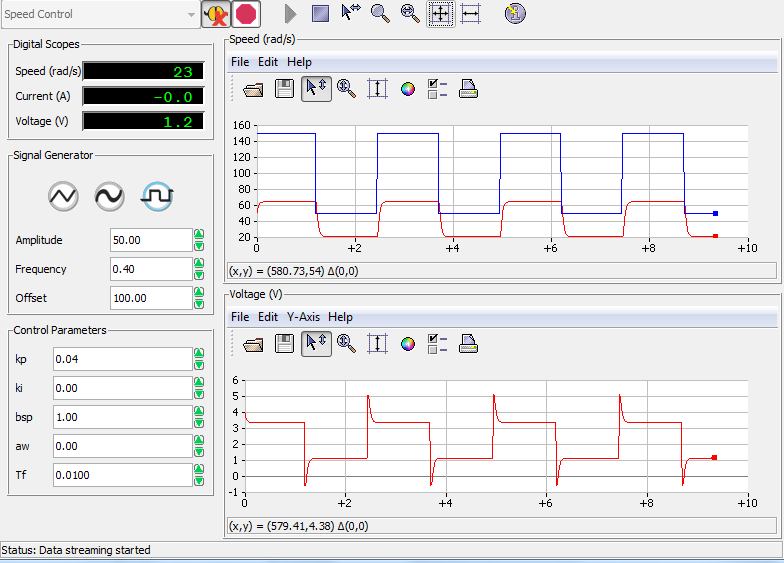
\includegraphics[width=6.50000in,height=4.66667in]{media/image39.png} \caption{Starting values for proportional control} \end{figure} 

\emph{Step 2: kp} from 0.1 V s/rad to 0.4 V s/rad, ki = 0

\begin{figure}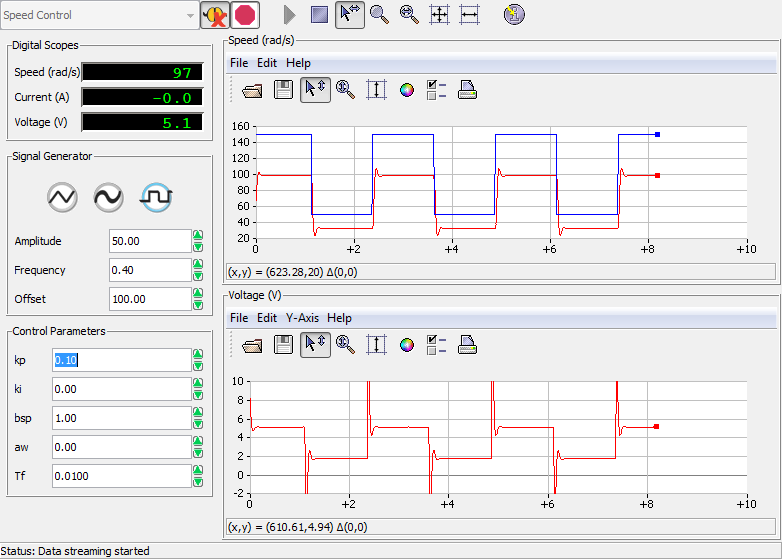
\includegraphics[width=6.50000in,height=4.65278in]{media/image37.png} \caption{$k_p = 0.1 \text{V s/rad }, k_i = 0$} \end{figure} 

Kp = 0.1 V s / rad

\begin{figure}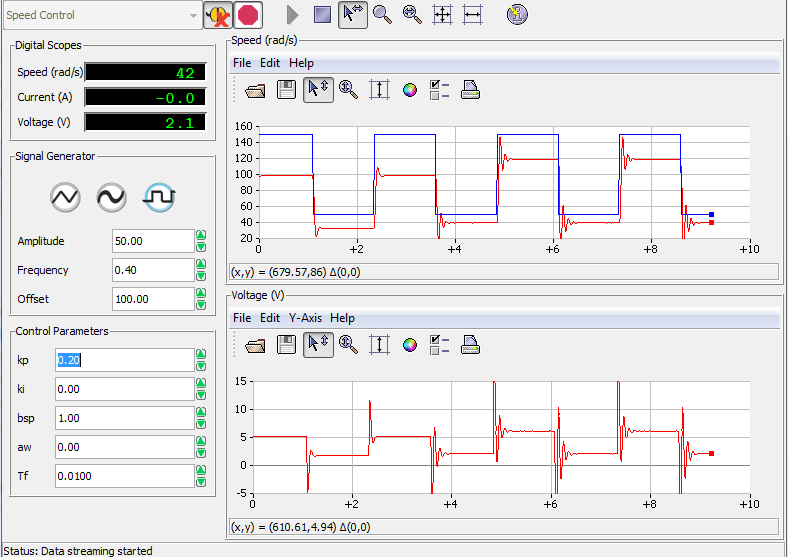
\includegraphics[width=6.50000in,height=4.59722in]{media/image56.png} \caption{$k_p = 0.2 \text{V s/rad}, k_i = 0$} \end{figure}

Kp = 0.2 V s /rad

\begin{figure}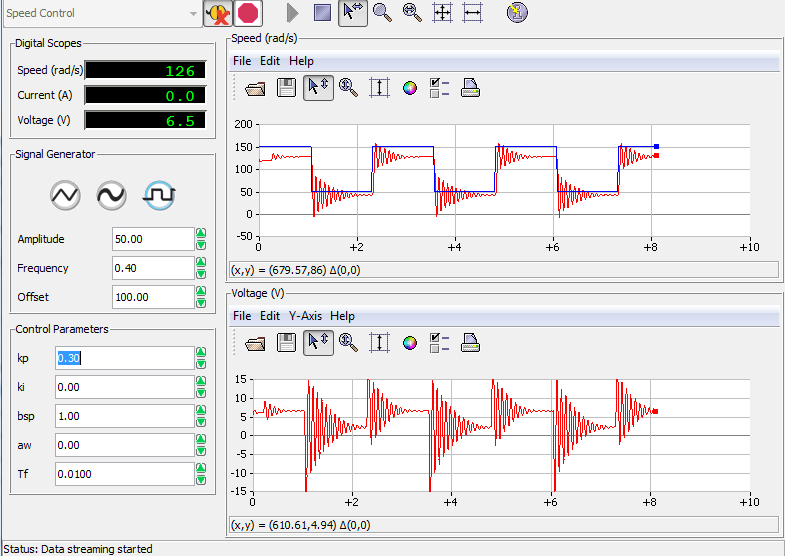
\includegraphics[width=6.50000in,height=4.59722in]{media/image60.png} \caption{$k_p = 0.3 \text{V s/rad } to, k_i = 0$} \end{figure}

Kp = 0.3 V s /rad

\begin{figure}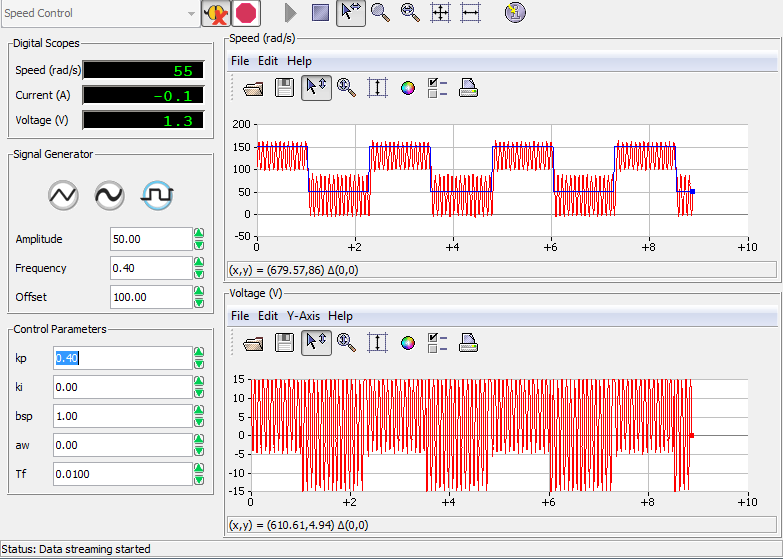
\includegraphics[width=6.50000in,height=4.63889in]{media/image16.png} \caption{$k_p = 0.4 \text{V s/rad }, k_i = 0$} \end{figure}
Kp = 0.4 V s /rad

Step 3 Observe and describe the steady-state error to a step input, as
\emph{kp} is increased

It decreased steady state

Step 4 Summarize your observations in your report and include some
representative results, screen captures, and plots. Discuss how your
plots compare with the analysis in 4.1.

Do later

\subsubsection{5.1.2. Integral Control}\label{integral-control}

Step 1 Set the proportional gain to zero. Set the integral gain to 0.4
V/rad to start with. Ensure that the parameters are set as listed in
Table 2.5.

\begin{figure}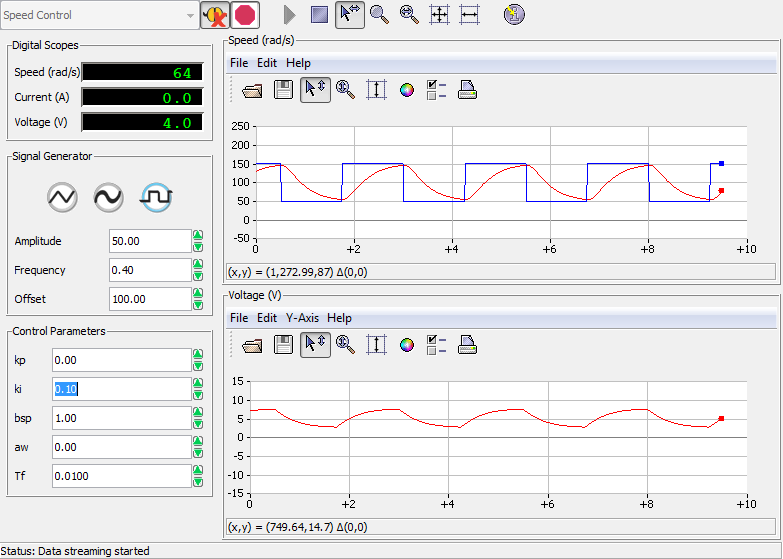
\includegraphics[width=6.50000in,height=4.63889in]{media/image59.png} \caption{$k_i = \text{0.1 V /rad}$} \end{figure}

Ki = 0.1 V /rad

\begin{figure}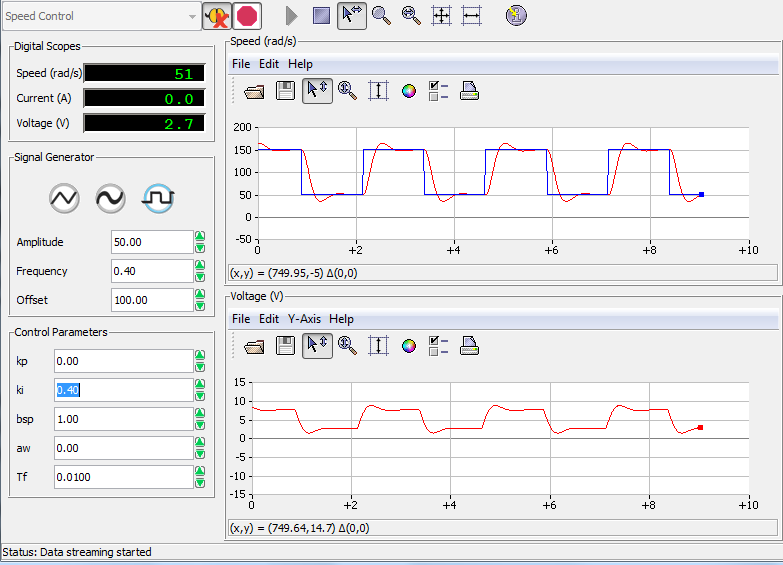
\includegraphics[width=6.50000in,height=4.69444in]{media/image43.png} \caption{$k_i = \text{0.4 V /rad}$} \end{figure}

Ki = 0.4 V/rad

\begin{figure}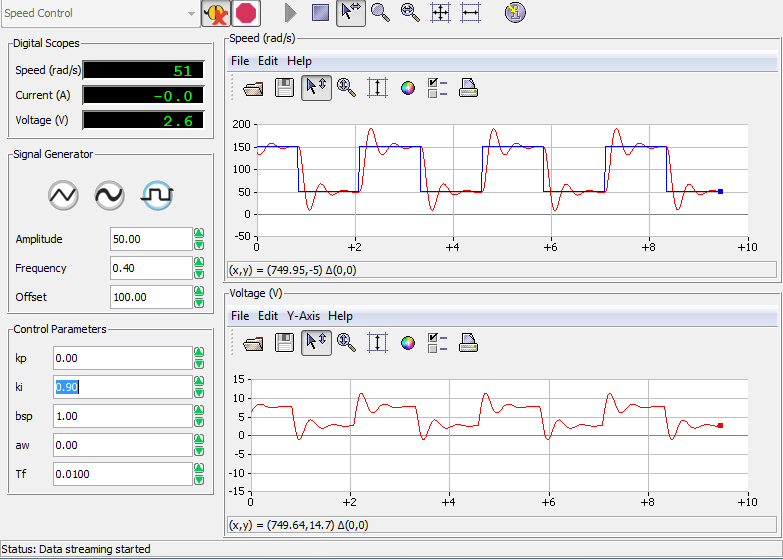
\includegraphics[width=6.50000in,height=4.65278in]{media/image12.png} \caption{$k_i = \text{0.9 V /rad}$} \end{figure}

Ki = 0.9 V rad

\begin{figure}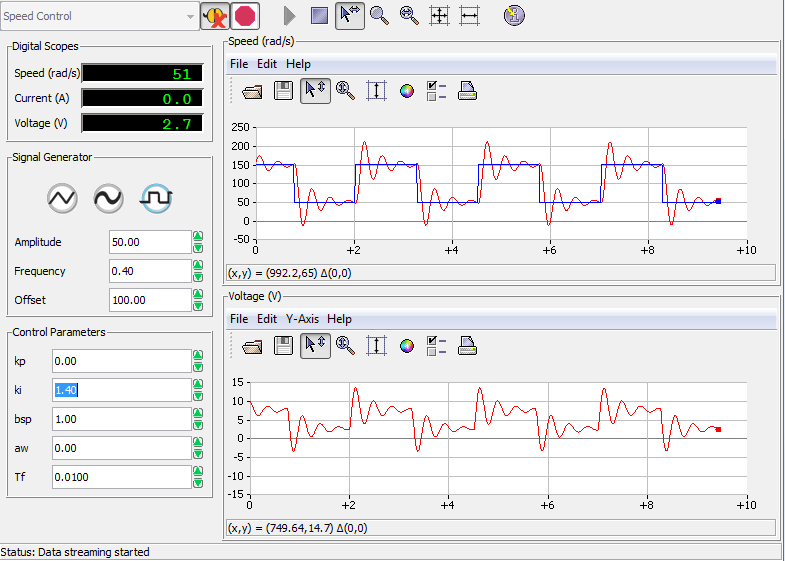
\includegraphics[width=6.50000in,height=4.63889in]{media/image11.png} \caption{$k_i = \text{1.4 V /rad}$} \end{figure}

ki = 1.4 V /rad

\begin{figure}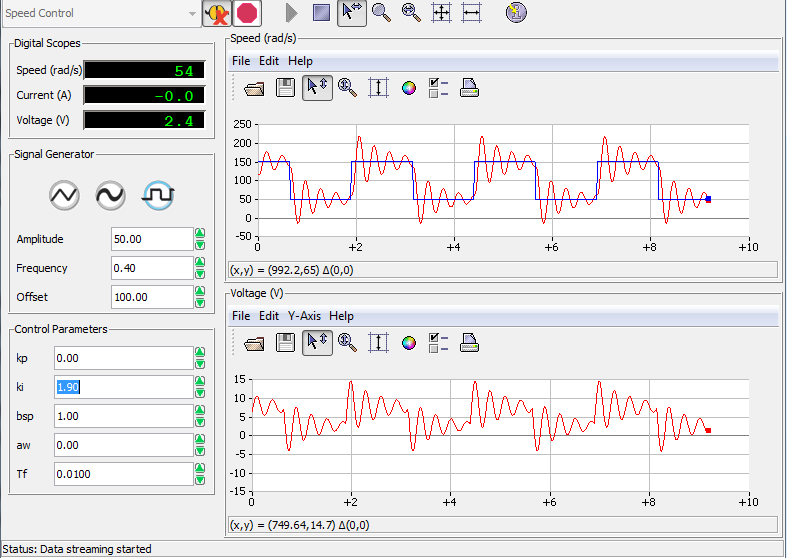
\includegraphics[width=6.50000in,height=4.61111in]{media/image47.png} \caption{$k_i = \text{1.9 V /rad}$} \end{figure}

Ki = 1.9 V /rad

Step 3 Determine a value of integral gain which gives the quickest
response without overshooting. Determine the settling time for this
closed loop system.

Ki should be about 0.16, and has no overshoot

\begin{figure}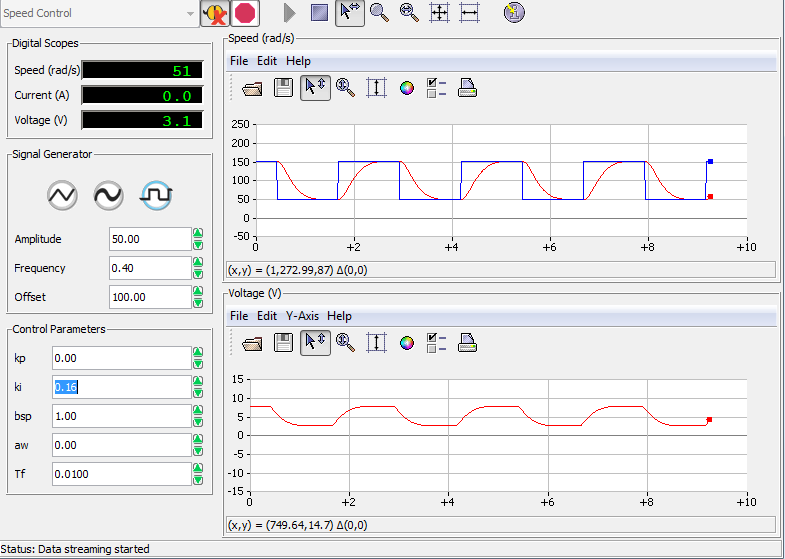
\includegraphics[width=6.50000in,height=4.62500in]{media/image40.png} \caption{$k_i = \text{0.16 V /rad}$} \end{figure}

Step 4 Summarize your observations in your report. Select some
representative results, screen captures, and plots. Discuss how your
plots compare with the analysis in 4.2.

Do later

\subsubsection{5.1.3. Proportional and Integral
Control}\label{proportional-and-integral-control}

The combination of proportional and integral control will now be
explored. Please follow the steps below.

Step 1. Set the parameters as listed in Table 2.6.

\begin{longtable}[]{@{}llll@{}}
\toprule
\emph{\textbf{Signal Type}} & \textbf{\emph{Amplitude} {[}rad/s{]}} &
\textbf{\emph{Frequency} {[}Hz{]}} & \textbf{\emph{Offset}
{[}rad/s\emph{{]}}}\tabularnewline
\midrule
\endhead
Square Wave & 50 & 0.4 & 100\tabularnewline
\bottomrule
\end{longtable}

Step 2. Set \emph{bsp} = 1, proportional gain to \emph{kp} = 0.1 V
s/rad, and change integral gain \emph{ki} in the range of 0.5 to 5
V/rad. Observe the tracking error (difference between input and output
signals) and the control signal.

Kp is constant

\begin{figure}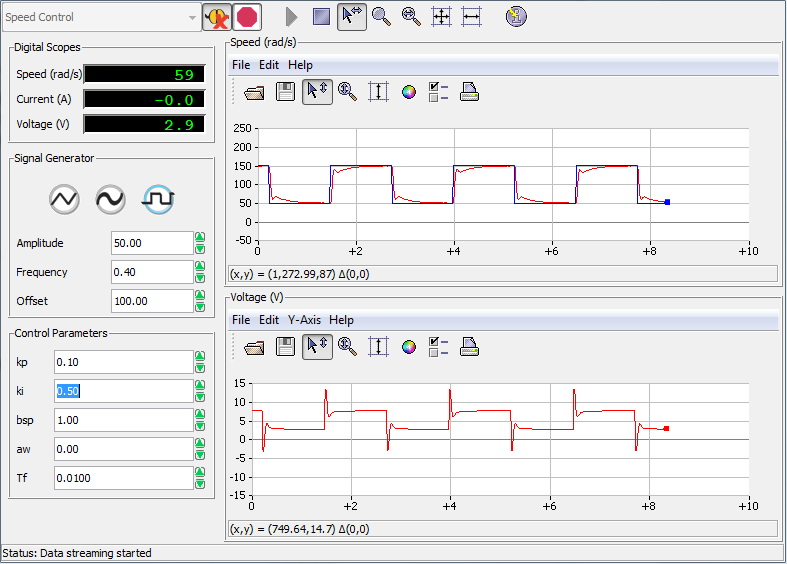
\includegraphics[width=6.50000in,height=4.65278in]{media/image57.png} \caption{$k_p = \text{0.1 V s /rad}, k_i = \text{0.5 V /rad}$} \end{figure}

Ki = 0.50 V /rad

\begin{figure}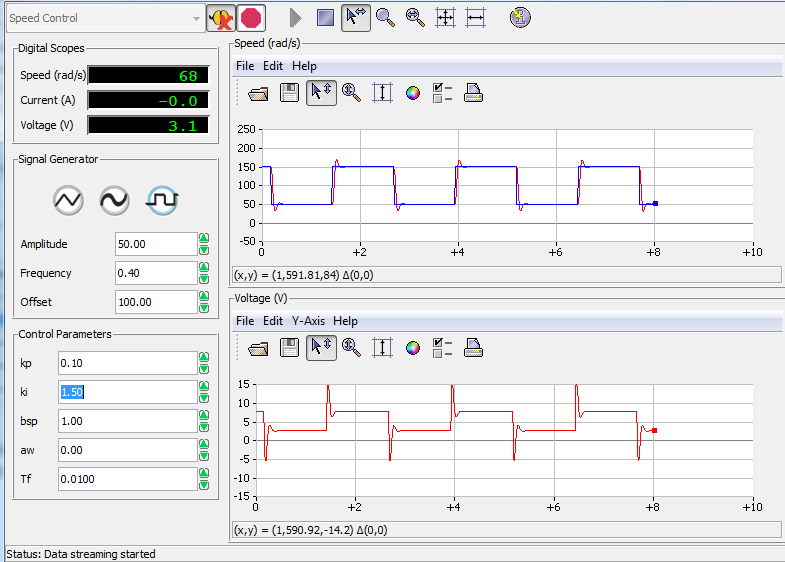
\includegraphics[width=6.50000in,height=4.65278in]{media/image58.png} \caption{$k_p = \text{0.1 V s /rad}, k_i = \text{1.5 V /rad}$} \end{figure}

Ki = 1.5 V/rad

\begin{figure}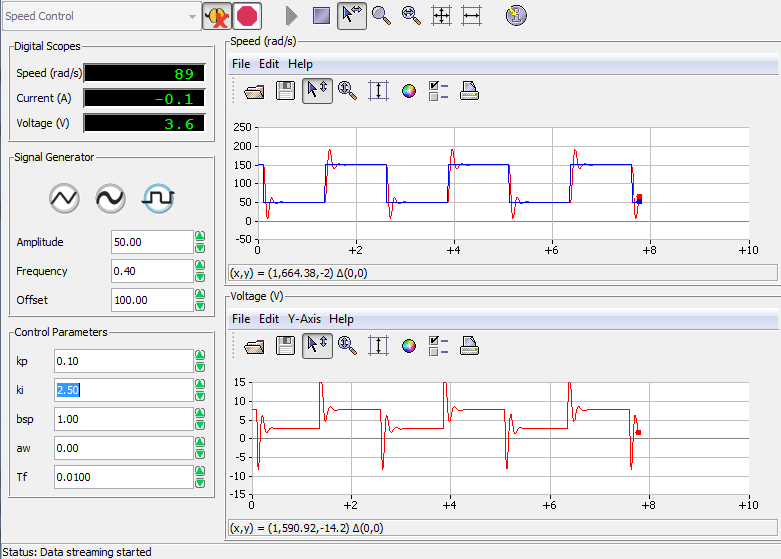
\includegraphics[width=6.50000in,height=4.65278in]{media/image14.png} \caption{$k_p = \text{0.1 V s /rad}, k_i = \text{2.5 V /rad}$} \end{figure}

Ki = 2.5 V/rad

\begin{figure}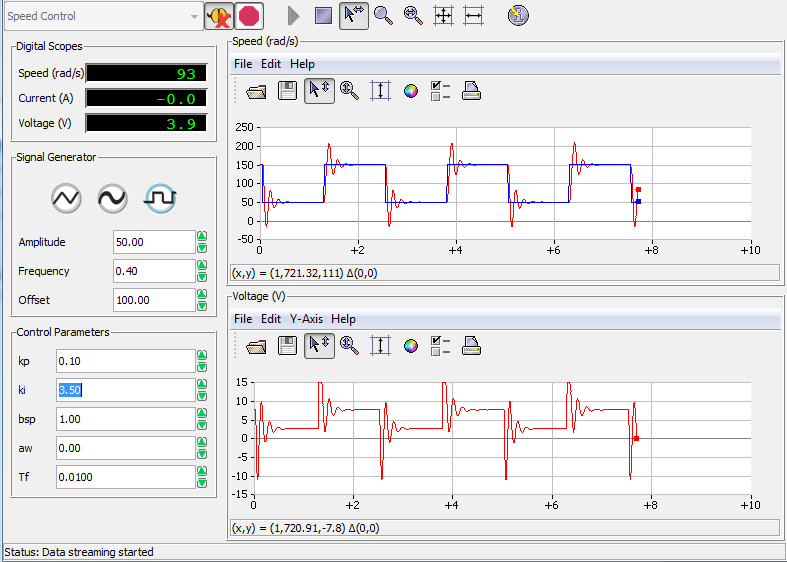
\includegraphics[width=6.50000in,height=4.63889in]{media/image49.png} \caption{$k_p = \text{0.1 V s /rad}, k_i = \text{3.5 V /rad}$} \end{figure}

Ki = 3.50 V / rad

\begin{figure}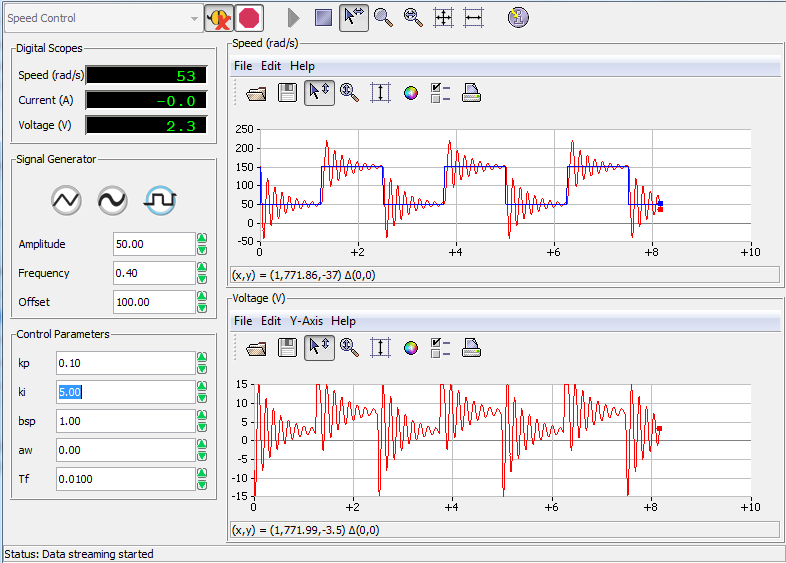
\includegraphics[width=6.50000in,height=4.65278in]{media/image51.png} \caption{$k_p = \text{0.1 V s /rad}, k_i = \text{5 V /rad}$} \end{figure}

Ki = 5 V /rad

Step 3. Set integral gain to \emph{ki} = 0.5 V/rad, \emph{bsp} = 1 and
change proportional gain \emph{kp} in the range of 0.05 to 0.3 V s/rad.
Observe the tracking error and the control signal.

\begin{figure}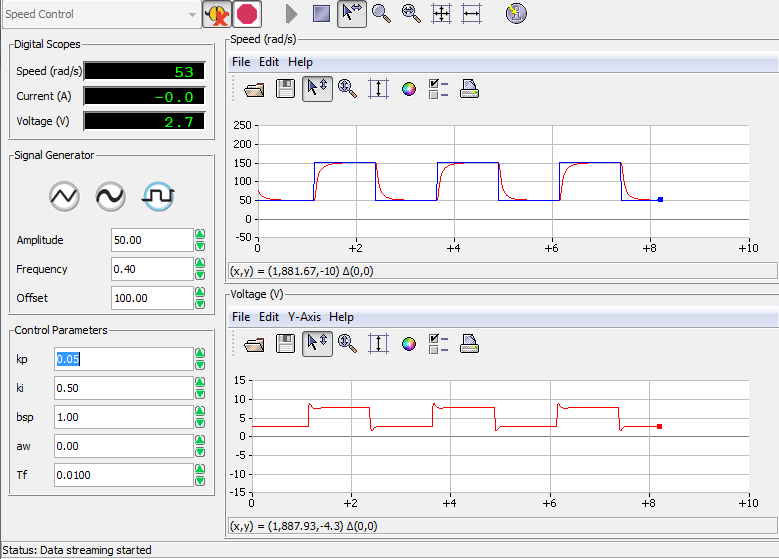
\includegraphics[width=6.50000in,height=4.66667in]{media/image29.png} \caption{$k_p = \text{0.05 V s /rad}, k_i = \text{0.5 V /rad}$} \end{figure}

Kp = 0.05 Vs /rad

\begin{figure}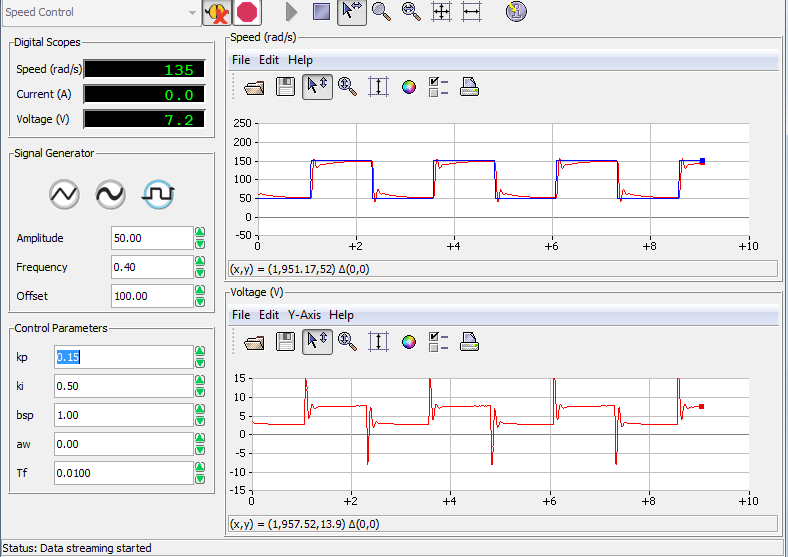
\includegraphics[width=6.50000in,height=4.59722in]{media/image9.png} \caption{$k_p = \text{0.15 V s /rad}, k_i = \text{0.5 V /rad}$} \end{figure}

Kp = 0.15 Vs /rad

\begin{figure}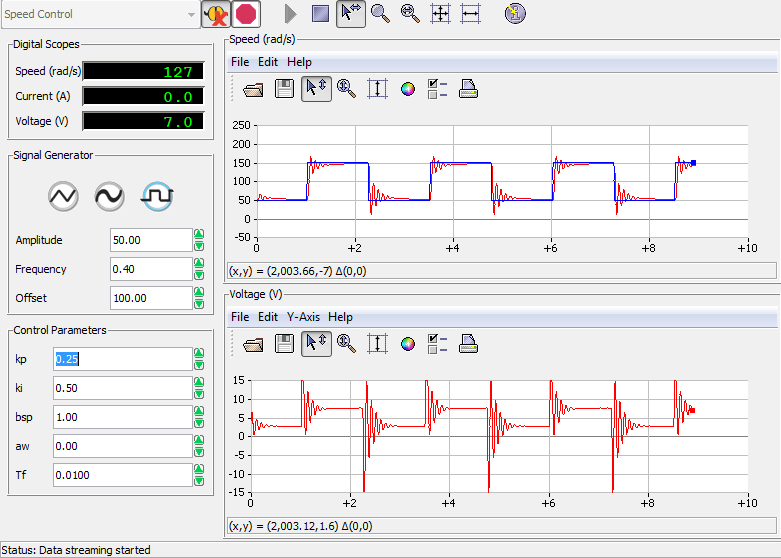
\includegraphics[width=6.50000in,height=4.63889in]{media/image18.png} \caption{$k_p = \text{0.25 V s /rad}, k_i = \text{0.5 V /rad}$} \end{figure}

Kp = 0.25 V s /rad

\begin{figure}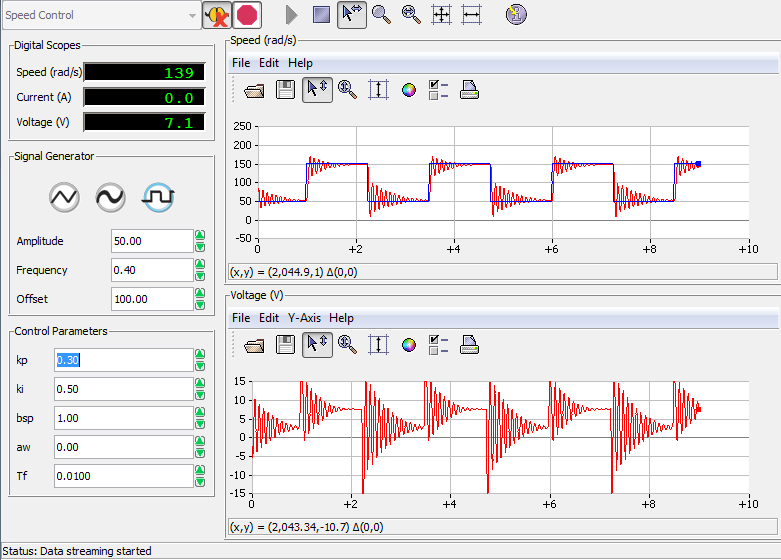
\includegraphics[width=6.50000in,height=4.66667in]{media/image32.png} \caption{$k_p = \text{0.30 V s /rad}, k_i = \text{0.5 V /rad}$} \end{figure}

Kp = 0.30 Vs /rad

Step 4. Set \emph{bsp}, the proportional and integral gains to the
values obtained in section 4.3.3. Observe the tracking error and the
control signal.

\begin{longtable}[]{@{}lll@{}}
\toprule
$b_sp$ =1 & $k_p$ = 0.10 Vs /rad & $k_i$=1.20 V /rad\tabularnewline
\bottomrule
\end{longtable}

\begin{figure}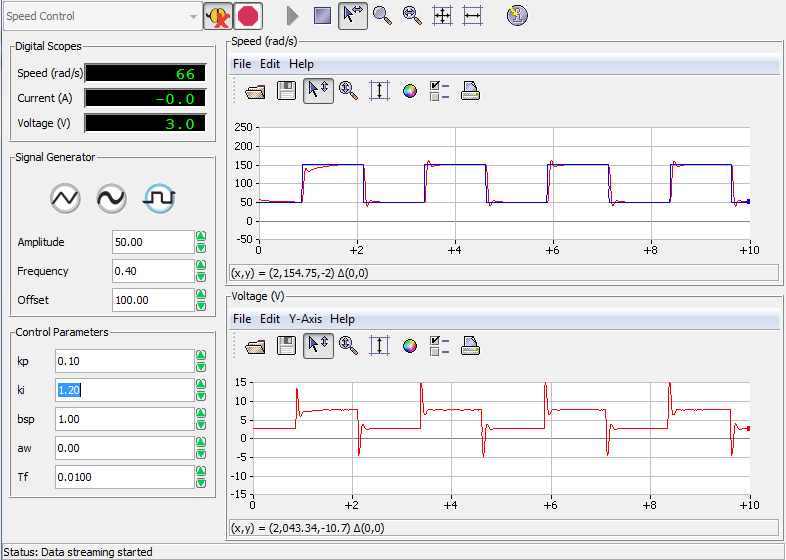
\includegraphics[width=6.50000in,height=4.62500in]{media/image35.png} \caption{$k_p = \text{0.1 V s /rad}, k_i = \text{0.5 V /rad}$} \end{figure}

Step 5. Summarize your observations in your report. Select some
representative results, screen captures, and plots. Discuss how your
plots compare with the analysis in 4.3.

Do later

\subsubsection{5.2. Close-loop System's Response to
Disturbances}\label{close-loop-systems-response-to-disturbances}

Step 1. The response to disturbance \emph{Td} at a constant reference
speed of 150 rad/s, is investigated. Set the signal generator module
parameters to 0 {[}rad/s{]} Amplitude and 150 {[}rad/s{]} Offset.

\begin{figure}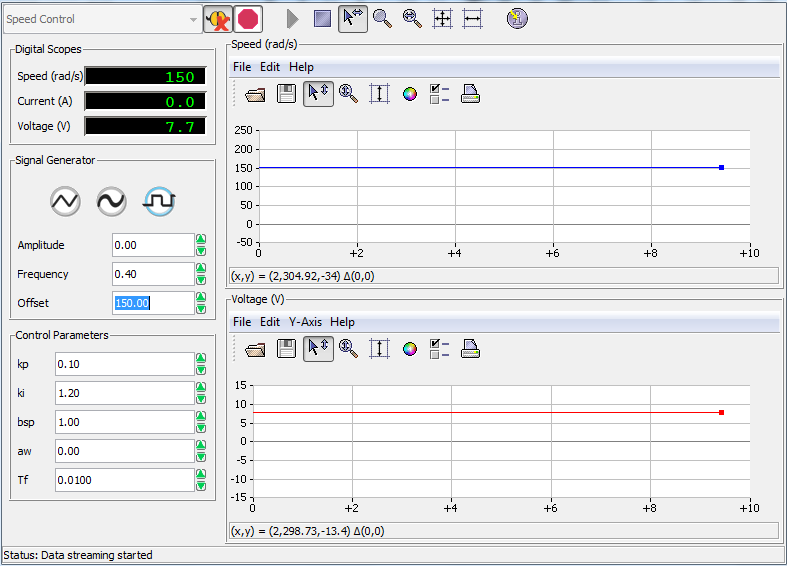
\includegraphics[width=6.50000in,height=4.68056in]{media/image48.png} \caption{Setting the Amplitude to 0 rad /s} \end{figure}

Step 2. Choose a pure proportional controller (\emph{ki} = 0, \emph{bsp}
= 1) with gain \emph{kp} = 0.20 Vs/rad. Apply a torque manually by
gently touching the inertial load with your finger. Observe what happens
when you change the gain of the controller.

\begin{figure}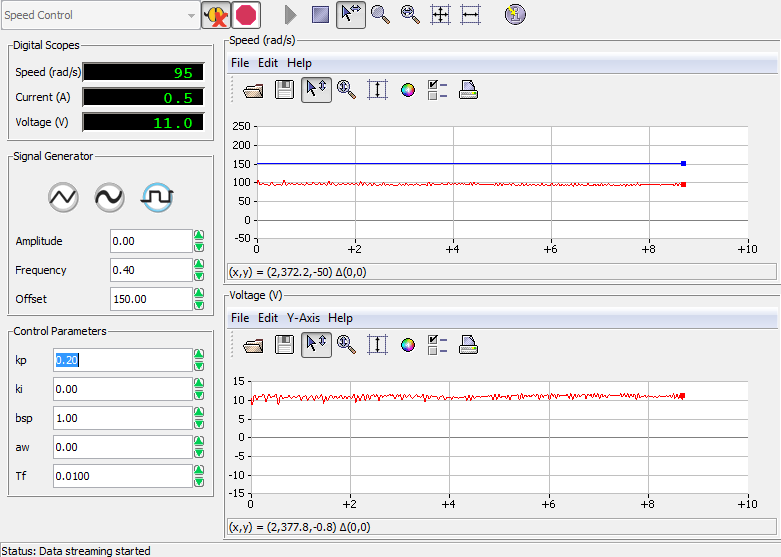
\includegraphics[width=6.50000in,height=4.63889in]{media/image22.png} \caption{Applying load with finger when $k_p = \text{0.2 V s /rad}, k_i = \text{0 V /rad}$} \end{figure}

Figure X : Gently touched motor with finger

\begin{figure}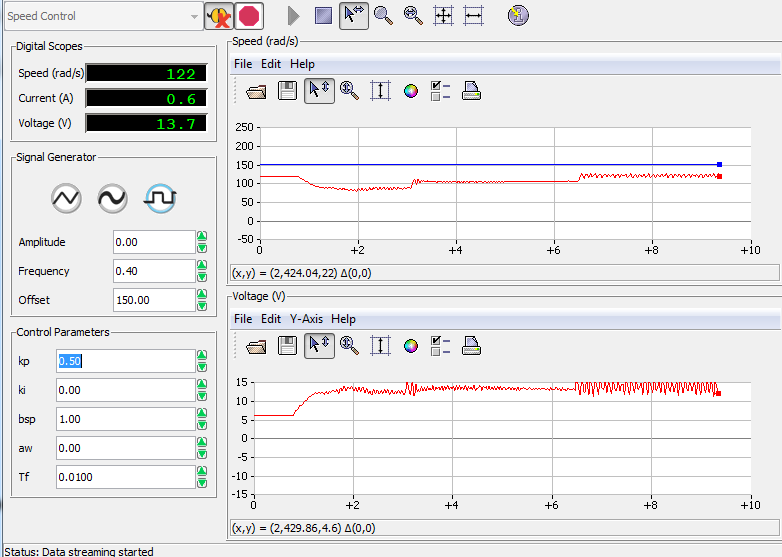
\includegraphics[width=6.50000in,height=4.62500in]{media/image19.png} \caption{Applying load with finger when $k_p = \text{0.5 V s /rad}, k_i = \text{0 V /rad}$} \end{figure}

Step 3. Choose a controller with pure integral action (\emph{kp} = 0),
such that ki = 1.0 V/rad. Apply a disturbance torque manually and
observe what happens.

\begin{figure}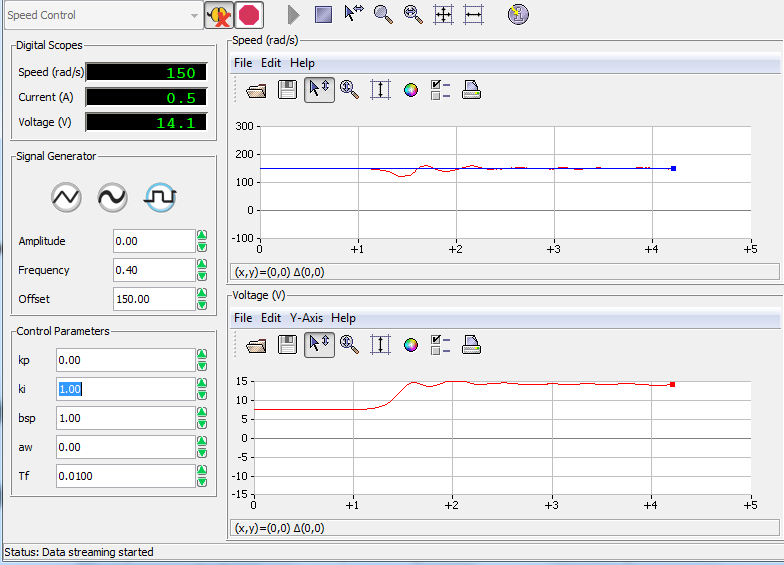
\includegraphics[width=6.50000in,height=4.68056in]{media/image33.png} \caption{Applying load with finger when $k_p = \text{0 V s /rad}, k_i = \text{1 V /rad}$} \end{figure}

Applying disturbance manually

Step 4. Observe the response of the system output w\emph{m} to the
external disturbance when using proportional control and when using
integral control. Summarize your observations and your calculations in
your report. Select some representative results, screen captures, and
plots.

\begin{figure}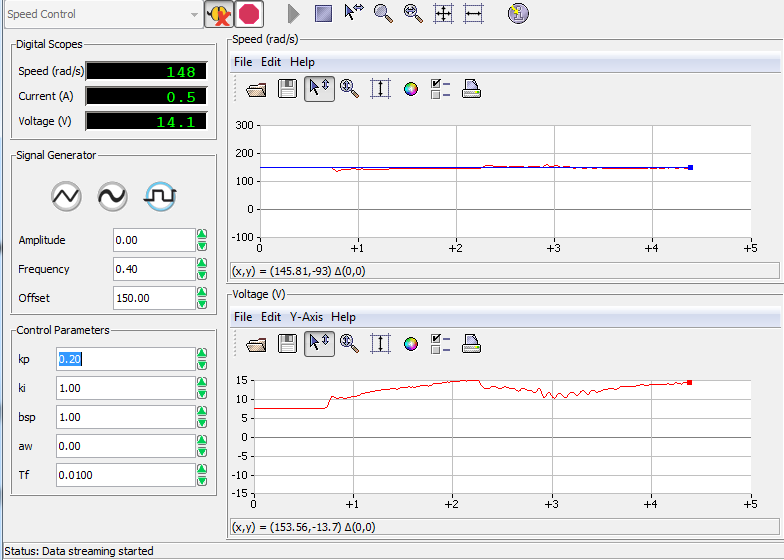
\includegraphics[width=6.50000in,height=4.63889in]{media/image26.png} \caption{Applying load with finger when $k_p = \text{0.2 V s /rad}, k_i = \text{1 V /rad}$} \end{figure}

Disturbance applied when using integral and proportional controller

\subsubsection{5.3. Manual Tuning of PI Controller:
Ziegler-Nichols}\label{manual-tuning-of-pi-controller-ziegler-nichols}

This part of the experiment should illustrate the performance of the
closed-loop system with a manually tuned PI controller and compare its
performance with the previous controllers.

Please follow the steps below.

Step 1. Determine the critical gain, \emph{kpc}, (\emph{ki} = 0,
\emph{bsp} = 1) where the system becomes critically stable and a stable
oscillation is achieved. Also determine the critical period \emph{Tpc}
of the corresponding oscillations (Refer to section 3.1 for procedures).
Using these values determine the Ziegler-Nichols controller gains using
the equations in 3.1.

\begin{figure}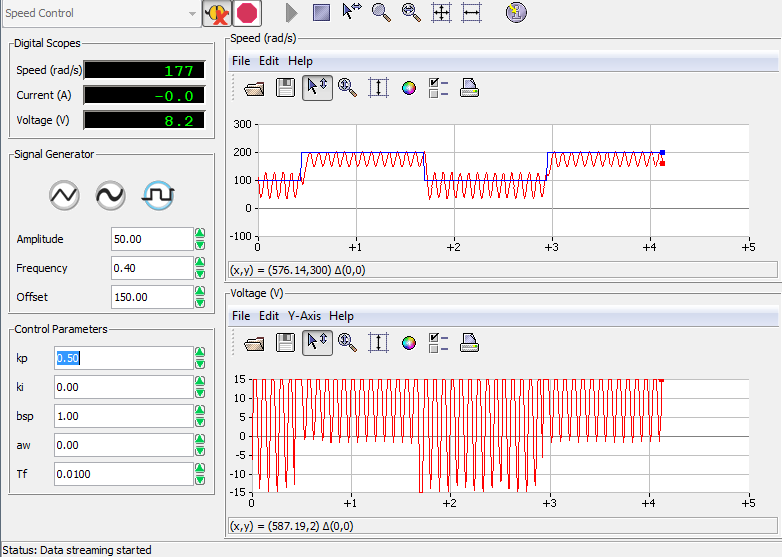
\includegraphics[width=6.50000in,height=4.62500in]{media/image30.png} \caption{Finding the value for critical gain, $k_{pc}$, manually.} \end{figure}

Finding a critical value for kp manually.

\begin{figure}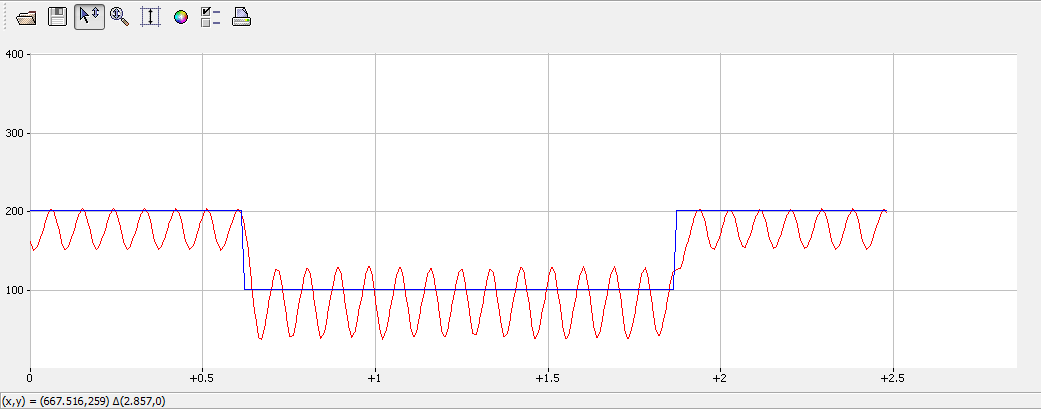
\includegraphics[width=6.50000in,height=2.55556in]{media/image50.png} \caption{Estimating the corresponding period, $T_{pc}$} \end{figure}

Finding the period for Tpc

\begin{table}
	\centering
	\begin{tabular}{llll}
		Description                & Symbol & In-Lab Result & Units  \\
		Properties of PI Control   &        &               &        \\
		Critical proportional gain & $k_{pc}$    & 0.5           & Vs/rad \\
		Critical period for kpc    & $T_{pc}$    & 0.9           & s      \\
		Ziegler-Nichols design     &        &               &        \\
		Proportional gain          & $k_p$     & 0.2           & Vs/rad \\
		Integral gain              & $k_i$    & 0.278         & V/rad  \\
	\end{tabular}
\end{table}

\emph{kp} = 0.4 \emph{kpc}

\emph{Ti} = 0.8 \emph{Tpc}

\emph{ki} = \emph{kp} / \emph{Ti} or \emph{ki} = 0.5 * \emph{kpc} /
\emph{Tpc}

Step 2. Set the parameters of the signal generator module window as
listed in Table 2.7.

\begin{longtable}[]{@{}llll@{}}
\toprule
\emph{\textbf{Signal Type}} & \textbf{\emph{Amplitude} {[}rad/s{]}} &
\textbf{\emph{Frequency} {[}Hz{]}} & \textbf{\emph{Offset}
{[}rad/s{]}}\tabularnewline
\midrule
\endhead
Square Wave & 50 & 0.5 & 150\tabularnewline
\bottomrule
\end{longtable}

\textbf{Table 2.7.} Module parameters for the Ziegler-Nichols-tuned PI
controller

Set \emph{bsp} = 1, both proportional and integral gains to their
Ziegler-Nichols values as calculated. above. What are your observations?

\begin{figure}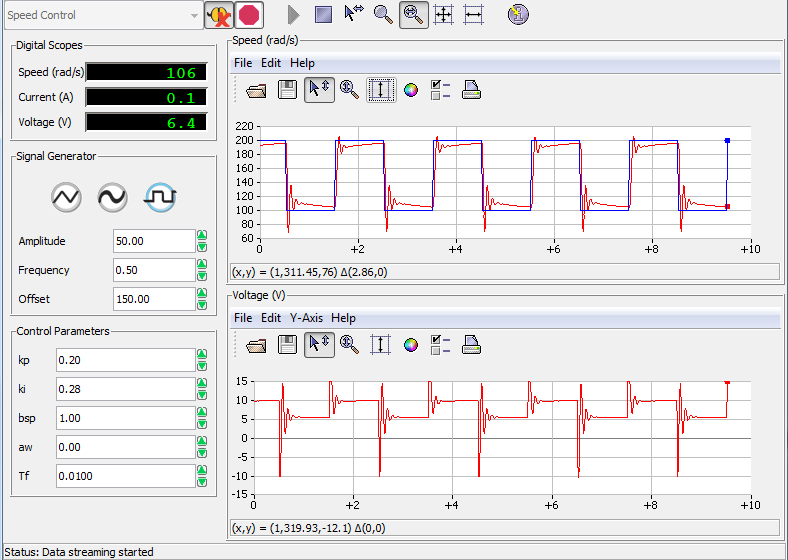
\includegraphics[width=6.50000in,height=4.62500in]{media/image44.png} \caption{Using the set values of $k_p = 0.2 Vs/rad $ and  $k_i = 0.278 V/rad$} \end{figure}

Figure X: Inputting values of Ziegler- Nichols Tuning

Step 3. Adjust proportional and integral gain manually to give a very
slightly under-damped response with no saturation of the control signal
(the system is saturated when changing the control signal does not have
any effect on the output signal). Comment on the new gain values.

\begin{figure}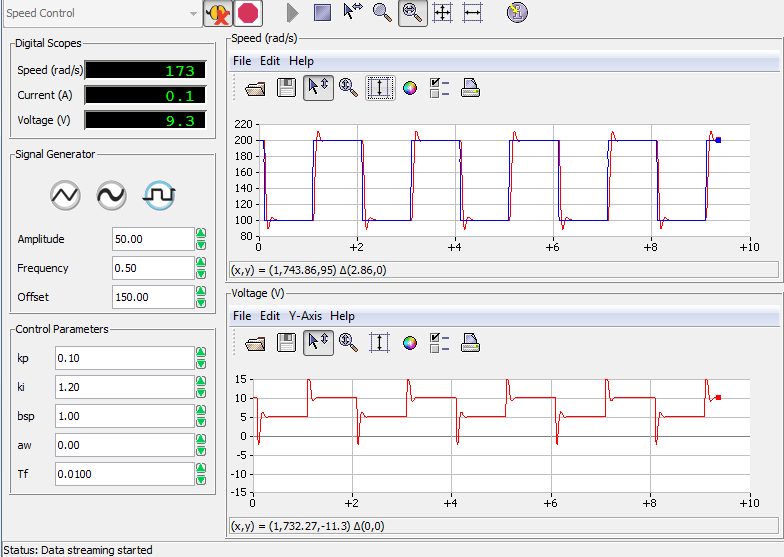
\includegraphics[width=6.50000in,height=4.61111in]{media/image25.png} \caption{Manually adjusted values until slightly underdamped response is reached.} \end{figure}

Figure X: manually tuning

Kp = 0.10 Vs /rad

Ki= 1.20 V /rad

Step 4. How does the response of the gain values of the Ziegler-Nichols
compare with the previous controllers in 5.1.1, 5.1.2. and 5.1.3.?
Explain your observations.

Step 5. Summarize your observations and your calculations in your
report. Select some representative results, screen captures, and plots.

\subsection{Discussion}\label{discussion}

\subsection{Conclusion}\label{conclusion}

\subsection{References}\label{references}

\begin{quote}
{[}1{]} Dr. P. Agathoklis et al. 2016. Laboratory Manual for ELEC 360
Control Systems I. University of Victoria, Canada.
\end{quote}

\end{document}
